\thispagestyle{plain}
\chapter{Evaluation}

This chapter will deal with the evaluation of the experiments

\section{Setup}
\begin{itemize}
    \item hardware
    \item index parameters like slot size, PGM epsilon etc.
\end{itemize}

\section{Datasets and Workloads}

\section{Role of Partitioning Parameters}
\begin{itemize}
    \item $$window_size$$, delta for frequency
    \item $$window_size$$ for purity (as of yet)
\end{itemize}

\section{Lookup Performance}

\subsection{Frequency Algorithm}

\subsection{Purity Algorithm}

\paragraph{Clear cuts experiment}

First of all, we conducted a rather simple experiment that was designed to confirm the result of \citeauthor{Dittrich2021} \cite{Dittrich2021}. While they hand crafted the boundaries, the partitions for the experiment here were generated by the purity partitioning algorithm. The workload that was executed on the data was split into three regions: the first 10 percent of the keys, the next 75 percent and finally the remaining 15 percent. The first region received 20 percent of the total queries as point queries, the second region received 10 percent of the queries as point queries and 20 percent as range queries. The final region received the remaining 50 percent of queries as point queries. For our experiment, we used 2 million queries in total of which 1 million served as a train workload and 1 million as a test workload. For the benchmarking on the test workload we therefore had the queries depicted in Table \ref{tab:poc_wkl}.

\begin{table}[H]
\centering
\begin{tabular}{rrrrr}
\hline
Region & from & to   & number queries & query type \\ \hline
1      & 0    & 0.1  & 200k           & Point      \\
2      & 0.1  & 0.85 & 100k           & Point      \\
2      & 0.1  & 0.85 & 200k           & Range      \\
3      & 0.85 & 1    & 500k           & Point      \\ \hline
\end{tabular}
\caption{Query Distribution for clear cuts experiment}
\label{tab:poc_wkl}
\end{table}

\begin{figure}[H]
    \centering
    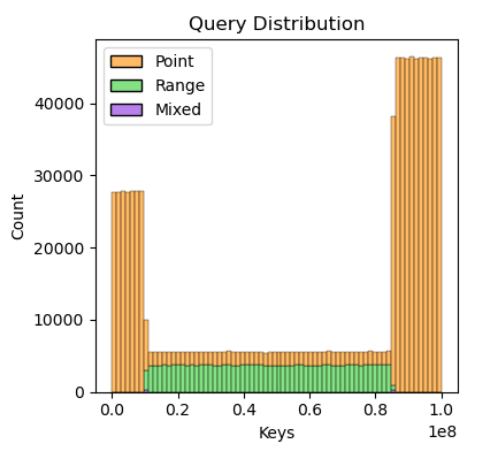
\includegraphics[width=0.6\textwidth]{figures/poc_dist.png}
    \caption{Query Distribution of clear cuts experiment over 100 million uniform dense keys}
    \label{fig:poc_dist}
\end{figure}

The resulting query distribution is visualized in Figure \ref{fig:poc_dist}. As we could already tell from the description of the query distribution, we have two very clear boundaries when looking at frequency as well as purity. While the first and last region are only requested by point queries, we can see that the middle part receives both types of queries. Notably, we see mostly orange and green bars in the figure in this region, as this range contains 75 million keys, but receives only 300 thousand queries. While there is some overlap of these queries, it is rather unlikely that one key from this range is selected for both point and range queries. This overlap would result in a purple bar in the figure. Nevertheless, a generalizing partitioning algorithm should recognize the boundaries and create three partitions accordingly.


//TODO: too small, make this bigger, maybe split single plots
\begin{figure}
    \centering
    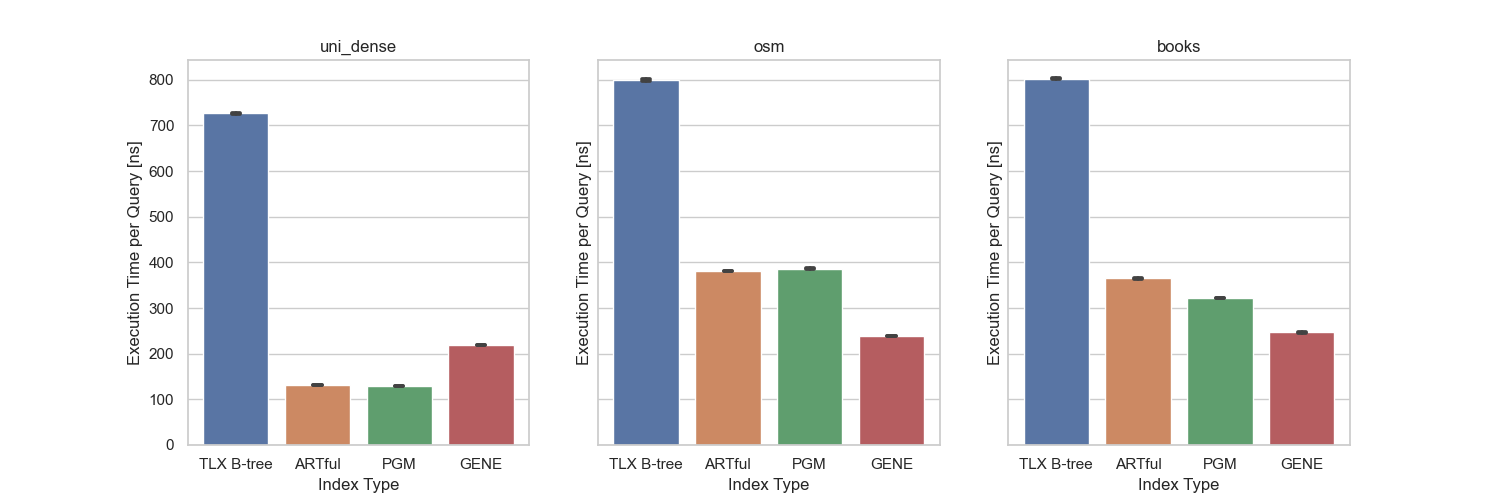
\includegraphics[width=\textwidth]{figures/poc_times.png}
    \caption{Average Query Execution Time on uniform dense data and the osm and books dataset}
    \label{fig:poc_times}
\end{figure}